\documentclass[11pt]{article}
\usepackage[T1]{fontenc}
\usepackage[utf8]{inputenc}
\usepackage{lmodern,microtype,amsmath,amssymb,amsthm,mathtools,mathrsfs}
\usepackage[margin=30mm]{geometry}
\usepackage{enumitem,booktabs}
\usepackage{tikz}
\usetikzlibrary{arrows.meta}
\usepackage[unicode,colorlinks=true,linkcolor=blue!45!black,urlcolor=blue!55!black,citecolor=green!35!black]{hyperref}
\usepackage{xcolor,xurl}
\setlength{\emergencystretch}{2em}
\numberwithin{equation}{section}
\newtheorem{theorem}{Theorem}[section]
\newtheorem{proposition}[theorem]{Proposition}
\newtheorem{lemma}[theorem]{Lemma}
\newtheorem{corollary}[theorem]{Corollary}
\theoremstyle{definition}\newtheorem{definition}[theorem]{Definition}
\theoremstyle{remark}\newtheorem{remark}[theorem]{Remark}
\title{Finite spectral evaluation and uniform filling bounds}
\author{}
\date{}
\begin{document}
\maketitle
\begin{abstract}
We study a finite functional on polynomials of degree less than $N$,
whose spectral nodes are the roots of $2T_N(z/2)+2$ and whose multiplier
is an integer Gaussian chirp. Double roots retain first derivatives;
the odd simple root has its own value term. We prove that the functional
has supremum-norm bound $1+|n|/2$, independently of the level $N$.
If the polynomial vanishes at every node, the bound improves to
$(N-1)/N$, independently also of the signed integer $n$. Tensor products
admit a further exact subtraction when only joint grid vanishing is
known. The proof uses canonical polynomial remainders, a finite midpoint
identity, and an explicit derivative interpolation formula. We also
construct a Fourier similarity between a concrete pair Casimir and its
polynomial face operator, so the resolvent reproduction identity holds
on the full matrix, including nilpotent parts. Regular confluent
specialization identifies the Gaussian multiplier with powers of an
explicit finite crossing matrix. For a planar diagram obtained from a
matched triangulated sphere, we prove that its reduced tensor evaluation
is one coefficient of the product of its local face polynomials. The
proof retains the actual cups, caps and marked cut, including the shifted
face lattice at even levels. An explicit matrix calculation identifies
the resulting knot evaluation with the reduced Kashaev invariant, up to
its stated unit framing factor. No volume asymptotic is assumed or proved.
\end{abstract}

\section{Introduction and the main estimate}

At a repeated spectral root, a polynomial is not determined by its
values. Its derivative can act on a nonzero nilpotent part of an
operator. This elementary fact matters when a crossing power is inserted
into a finite spectral source: a value-only sum would omit some of the
original matrix entries. The purpose of this paper is to retain those
entries while bounding the insertion by the supremum of the original
polynomial on a real interval. We then prove the exact diagram identity
needed to apply that bound: the face variables shared by different
crossings are identified before taking the prescribed coefficient.

Fix $N\ge2$, and write
\[
 d=N-1,\qquad q=e^{\pi i/N},\qquad Q=q^2,\qquad
 \chi_N(z)=2T_N(z/2)+2.
\]
The Chebyshev polynomial is defined by $T_N(\cos\phi)=\cos(N\phi)$;
$\chi_N$ is monic of degree $N$. Its distinct double roots are
\[
 c_a=2\cos\frac{(2a+1)\pi}{N},\qquad
 0\le a<\lfloor N/2\rfloor.
\]
For odd $N$ there is one further root, $-2$, of multiplicity one.
All statements below apply to both parities and to composite levels.

Let $\mathcal R_{\chi_N}F$ be the canonical polynomial remainder modulo
$\chi_N$, and put
\[
 \ell_N(F)=[z^{N-1}]\mathcal R_{\chi_N}F.
\]
For $n\in\mathbb Z$, the multiplier $f_n$ is specified at the spectral
roots by the local germs
\[
 f_n(2\cos\phi)=q^{nd^2/4}
       \exp\!\left(\frac{inN(\phi-\pi)^2}{4\pi}\right),
       \qquad 0<\phi<2\pi.
\]
The formula is symmetric about $\pi$ and defines a regular germ at
$z=-2$. Its Hermite polynomial $\widetilde f_n$ is the unique polynomial
of degree less than $N$ with those values and first derivatives at the
double roots, and the specified value at the odd simple root. Define
\[
             \mathcal L_N^nH=\ell_N(\widetilde f_nH).
\]
The product is taken before reduction. In particular $\ell_N$ is not
being treated as a multiplicative functional.

\begin{theorem}[Uniform finite filling bound]\label{fb:main}
For every complex polynomial $H$ of degree at most $d$ and every signed
integer $n$,
\begin{equation}\label{uf:eq-1}
 |\mathcal L_N^nH|\le(1+|n|/2)\|H\|_{[-2,2]}.
\end{equation}
If $H$ vanishes at all distinct roots of $\chi_N$, then
\begin{equation}\label{uf:eq-2}
 |\mathcal L_N^nH|\le(d/N)\|H\|_{[-2,2]}.
\end{equation}
For a polynomial $S$ in $r$ spectral variables, of degree at most $d$
in each variable, suppose that it vanishes whenever $\sigma_e$ is a
spectral node, with the other variables arbitrary, for each $e$ in a
set $J$. Then
\begin{equation}\label{uf:eq-3}
 \left|\left(\bigotimes_{e=1}^r\mathcal L_N^{n_e}\right)S\right|
 \le(d/N)^{|J|}\prod_{e\notin J}(1+|n_e|/2)\,
                         \|S\|_{[-2,2]^r}.
\end{equation}
Finally, if $\mathcal D$ has the same degree bounds and vanishes only
on the Cartesian product of all node sets, then
\begin{equation}\label{uf:eq-4}
 \left|\left(\bigotimes_{e=1}^r\mathcal L_N^{n_e}\right)\mathcal D\right|
 \le\left\{\prod_e(1+|n_e|/2)
       -\prod_e(1/N+|n_e|/2)\right\}\|\mathcal D\|_{[-2,2]^r}.
\end{equation}
\end{theorem}

Here $\|H\|_{[-2,2]}=\max_{-2\le x\le2}|H(x)|$, and the cube norm
has the analogous meaning. The tensor product denotes successive
application in the separate spectral variables. These operations
commute because they act in different scalar variables; this says
nothing about commutation of matrices at different crossings.

The derivative inequality used below is the classical Bernstein
inequality, obtained here from Riesz's finite interpolation formula
\cite{Riesz1914}. The interpolation and polynomial-division tools
are standard. The calculations in this paper specify their application
to the stated Gaussian Hermite functional, with its normalization
and tensor-grid subtraction.

The proof of the theorem occupies Sections~\ref{uf:sec-repeated-roots-the-odd-simple-root-and-the-midpoint-identity}--\ref{uf:sec-shared-polynomials-and-the-unsplit-complementary-source}.
Its essential estimate is a finite derivative formula with total
coefficient mass $d$. Thus the constant is independent of the number
of interpolation nodes, even though the functional retains derivatives
at nearly every distinct root. The degree restriction is essential to
this argument and will be retained in every application.

The knot-theoretic motivation is the relation between root-of-unity
quantum invariants and hyperbolic volume initiated by Kashaev
\cite{Kashaev1997} and Murakami--Murakami \cite{MurakamiMurakami2001}.
The present theorem is a finite estimate. It separates the cost of
inserting fixed crossing powers from the harder problem of estimating
a shared source polynomial. Section~\ref{de:section} proves the global
coefficient identity, including the turns, the reduced mark and the face
lattice. Section~\ref{de:normalization-section} compares its literal
crossing matrices and normalization with the reduced Kashaev invariant.
The last section states the remaining asymptotic implication: a nonzero
leading contribution and a strict bound for the entire remainder give
the rate of the full invariant. Those analytic estimates and the
identification of their rate with hyperbolic volume are not proved here.

\section{Polynomial reduction and resolvent reproduction}
\label{uf:sec-canonical-reduction}

The value-and-derivative interpolation is the classical construction
of Hermite~\cite{Hermite1878}. We record its elementary polynomial
form, including repeated roots, because it fixes the coefficient
functional used here. Before using the particular spectral roots,
we record the algebraic
fact behind reduction at repeated roots. It explains which parts of the
calculation depend only on the polynomial and which still require the
original crossing operator.

Let \(R\) be a commutative ring with identity, and let
\(r_1,\ldots,r_m\in R\), with \(m\ge1\). Repetitions are allowed.
Put \(p(X)=\prod_{j=1}^m(X-r_j)\). Given \(f\in R[X]\), define
\(f_0=f\) and successively define \(f_j\) by
\[
 f_{j-1}(X)=f_{j-1}(r_j)+(X-r_j)f_j(X),\qquad 1\le j\le m.
\]
Each \(f_j\) is obtained by synthetic division. This is a polynomial
operation: it uses no inverse in \(R\), even if two roots coincide.
Define
\[
 \mathcal R_p f(X)=
 \sum_{j=1}^m f_{j-1}(r_j)\prod_{i<j}(X-r_i),
 \qquad
 \ell_p(f)=[X^{m-1}]\mathcal R_p f.
\]
Here \([X^k]\) means the coefficient of \(X^k\), and an empty
product is one.

\begin{proposition}[Canonical polynomial remainder]
\label{prop:canonical-polynomial-remainder}
The polynomial \(\mathcal R_p f\) is the unique polynomial of degree
less than \(m\) for which \(f-\mathcal R_p f\) is a multiple of
\(p\). Consequently it is independent of the ordering of the root
list, including repeated entries. Both \(\mathcal R_p\) and
\(\ell_p\) are \(R\)-linear, and adding a multiple of \(p\) to
their input leaves their values unchanged. Moreover,
\[
 \ell_p(f)=f_{m-1}(r_m).
\]
Among additive functionals on \(R[X]\), \(\ell_p\) is uniquely
specified by the two requirements
\[
 F(pq)=0\quad\text{for every }q\in R[X],\qquad
 F(r)=[X^{m-1}]r\quad\text{whenever }\deg r<m.
\]
\end{proposition}

\begin{proof}
Substituting each synthetic-division identity into the preceding one
gives \(f=p f_m+\mathcal R_p f\). Every summand in the displayed
remainder has degree at most \(m-1\). If two such remainders existed,
their difference would have degree less than \(m\) and would be a
multiple of the monic polynomial \(p\). A nonzero multiple \(pq\)
has degree \(m+\deg q\): its leading coefficient is the leading
coefficient of \(q\), because that of \(p\) is one. This argument
works even when \(R\) has zero divisors. The difference must therefore
vanish.

Uniqueness proves independence of root order, linearity and invariance
under adding a multiple of \(p\). In the Newton expression for the
remainder, only the last summand can contribute to \(X^{m-1}\);
its product of linear factors is monic. This proves the formula for
\(\ell_p\). Finally, any additive \(F\) with the two stated
properties satisfies
\[
 F(f)=F(pf_m)+F(\mathcal R_p f)
      =[X^{m-1}]\mathcal R_p f=\ell_p(f).
\]
\end{proof}

For two equal roots this construction gives
\[
 \mathcal R_{(X-r)^2}f(X)=f(r)+f'(r)(X-r),
 \qquad \ell_{(X-r)^2}(f)=f'(r).
\]
The derivative is the formal polynomial derivative. Thus repeated
roots retain derivative information; replacing them by a single
evaluation changes the operation.

\begin{proposition}[Products and repeated-root derivatives]
\label{prop:canonical-remainder-products}
For any $f,g\in R[X]$,
\[
 \mathcal R_p(fg)=
 \mathcal R_p\bigl((\mathcal R_p f)(\mathcal R_p g)\bigr),
 \qquad
 \ell_p(fg)=\ell_p\bigl((\mathcal R_p f)(\mathcal R_p g)\bigr).
\]
Consequently a finite product may be reduced after each multiplication,
with the same final remainder and coefficient functional. This reduced
multiplication is associative. If $r$ occurs at least twice among the
roots of $p$, the final remainder retains both $(fg)(r)$ and
\[
 (fg)'(r)=f'(r)g(r)+f(r)g'(r).
\]
For the modulus $(X-r)^2$ its full expression is
\[
 \mathcal R_{(X-r)^2}(fg)
 =f(r)g(r)+\bigl(f'(r)g(r)+f(r)g'(r)\bigr)(X-r).
\]
No degree bound on the unreduced factors or their product is required.
\end{proposition}

\begin{proof}
Write $f=\mathcal R_p f+pa$ and $g=\mathcal R_p g+pb$ using
synthetic division. Their product differs from
$(\mathcal R_p f)(\mathcal R_p g)$ by
$p\{a\mathcal R_p g+b\mathcal R_p f+pab\}$. Uniqueness of the
remainder proves the first equality; taking its top coefficient proves
the second. Repeating the equality proves the finite-product statement.
Either parenthesization of a product of three factors reduces the same
polynomial $fgh$, which proves associativity.

When $(X-r)^2$ divides $p$, the difference between any polynomial and its
remainder has both value and formal derivative zero at $r$. The formal
product rule gives the displayed derivative. The explicit degree-one
remainder then follows from the double-root formula above.
\end{proof}

The coefficient functional is linear, but it is generally not
multiplicative: $\ell_p(fg)$ need not equal $\ell_p(f)\ell_p(g)$.
The product must be formed and reduced before its coefficient is taken.
At a repeated spectral root the product rule also retains the first
derivative of either factor; a list of values alone cannot replace it.
This permits a product of arbitrary degree to be formed first and
reduced only when the coefficient functional is applied.

There is also a direct algebraic relation between this coefficient
functional and the resolvent numerator. It does not require a
diagonalization of the operator.

\begin{proposition}[Reproduction by the polynomial resolvent]
\label{prop:resolvent-reproduction}
Let \(p(X)\) be a split monic polynomial of degree \(m\ge1\)
over a commutative algebra \(A\), and let \(w\in A\) satisfy
\(p(w)=0\). Define \(V_w\) by polynomial synthetic division,
\[
 V_w(X)=\frac{p(X)-p(w)}{X-w}.
\]
The fraction denotes a polynomial, with no inverse assumed in \(A\).
Let \(\ell_p\) be the coefficient of \(X^{m-1}\) in the
canonical remainder modulo \(p\). For every \(f\in A[X]\),
\[
                   \ell_p(fV_w)=f(w).
\]
Repeated roots of \(p\) are allowed.
\end{proposition}

\begin{proof}
Synthetic division gives \((X-w)V_w=p\). The polynomial \(V_w\)
is monic of degree \(m-1\), so \(\ell_p(V_w)=1\).
For every polynomial \(g\), the identity
\((X-w)gV_w=pg\) and the vanishing of \(\ell_p\) on multiples
of \(p\) imply
\[
               \ell_p(XgV_w)=w\ell_p(gV_w).
\]
Induction gives \(\ell_p(X^jV_w)=w^j\). Linearity proves the
claim for arbitrary \(f\), with no restriction on its degree.
\end{proof}

For a matrix application, use the commutative algebra generated by
one matrix $\Omega$ and scalar matrices. If $p(\Omega)=0$, then the
proposition applies with $w=\Omega$ and gives the full matrix $f(\Omega)$,
including its nilpotent part. No diagonalization is required. A concrete
Casimir matrix satisfying the required relation is treated in
Section~\ref{uf:local-fourier}.

\section{Repeated roots, the odd simple root, and the midpoint
identity}\label{uf:sec-repeated-roots-the-odd-simple-root-and-the-midpoint-identity}

For completeness, the recurrence $2T_{j+1}(z/2)=z\,2T_j(z/2)-2T_{j-1}(z/2)$
shows that $\chi_N$ is monic of degree $N$. In the variable $\phi$,
$\chi_N(2\cos\phi)=2\cos(N\phi)+2$ has a double zero whenever
$N\phi$ is an odd multiple of $\pi$. Away from $\phi=\pi$ the
change of variable has nonzero derivative, so these give double roots
in $z$. For odd $N$, near $\phi=\pi+t$ one has
$\chi_N(2\cos\phi)=N^2t^2+O(t^4)$ and
$2\cos\phi+2=t^2+O(t^4)$, giving the simple root $-2$.
The resulting multiplicities add to $N$, so there are no others.

Write \begin{equation}\label{uf:eq-8}
c_a=2\cos\frac{(2a+1)\pi}{N},\qquad
 0\le a<\lfloor N/2\rfloor.
\end{equation} These are the distinct double roots. The only remaining root is
\(-2\), simple, when \(N\) is odd. At a double root \(c\), put
\(h(z)=\chi_N(z)/(z-c)^2\). The Chebyshev differential equation gives \begin{equation}\label{uf:eq-9}
h(c)=\frac{N^2}{4-c^2},\qquad
 \frac{h'(c)}{h(c)}=\frac{c}{4-c^2};
 \qquad \chi_N'(-2)=N^2\quad(N\ \mathrm{odd}).
\end{equation} Indeed \((4-z^2)\chi_N''-z\chi_N'+N^2(\chi_N-2)=0\). Evaluate it and
its derivative at \(c\), using \(\chi_N(c)=\chi_N'(c)=0\), to obtain
\eqref{uf:eq-9}.

The formula for the coefficient functional follows directly from
partial fractions. For a polynomial $F$, replace it by its remainder
$r=\mathcal R_{\chi_N}F$, of degree less than $N$. The coefficient of
$z^{-1}$ in $r(z)/\chi_N(z)$ at infinity is $\ell_{\chi_N}(F)$.
At a double root $c$, the coefficient of $(z-c)^{-1}$ is
\[
 \left(\frac r h\right)'(c)
 =\frac{r'(c)}{h(c)}-\frac{h'(c)r(c)}{h(c)^2}.
\]
At the odd simple root it is $r(-2)/\chi_N'(-2)$. Summing these
coefficients and using \eqref{uf:eq-9} gives
\begin{equation}\label{uf:eq-10}
\mathcal L_N^fH=
 \sum_a\frac{(4-c_a^2)(fH)'(c_a)-c_af(c_a)H(c_a)}{N^2}
 +\mathbf1_{N\ \mathrm{odd}}\frac{f(-2)H(-2)}{N^2}.
\end{equation}
Here $f$ may be a specified holomorphic germ at each root. Its Hermite
polynomial is the unique polynomial of degree less than $N$ with those
values and first derivatives at the double roots, and its value at the
odd simple root. Existence follows because the corresponding linear map
between two $N$-dimensional spaces has zero kernel: a polynomial with
all these jets zero is divisible by the monic degree-$N$ polynomial
$\chi_N$. We define $\mathcal L_N^fH=\ell_{\chi_N}(\widetilde f H)$,
where $\widetilde f$ is that Hermite polynomial. Formula \eqref{uf:eq-10}
therefore applies to every polynomial $H$, without choosing a global
branch for $f$. Its prime denotes differentiation in $z$.

Let \begin{equation}\label{uf:eq-11}
\phi_k=\frac{(2k+1)\pi}{N},\quad 0\le k<N,\qquad
 P(\phi)=H(2\cos\phi).
\end{equation} Each double root appears twice in this grid. At the odd simple root,
\(\phi=\pi\) occurs once, and differentiating the sine supplies exactly
its weight in \eqref{uf:eq-10}. Thus \eqref{uf:eq-10} is equivalently \begin{equation}\label{uf:eq-12}
\mathcal L_N^fH
 =-\frac1{2}\sum_{k=0}^{N-1}
       \left.\frac{d}{d\phi}
       \frac{2\sin\phi\,f(2\cos\phi)H(2\cos\phi)}{N^2}
       \right|_{\phi=\phi_k}.
\end{equation} There is no omission or doubling of the odd simple node.

For the integer $n$ in Theorem~\ref{fb:main}, the centered Gaussian
is \begin{equation}\label{uf:eq-13}
f_n(2\cos\phi)=q^{nd^2/4}
          \exp\left(\frac{inN(\phi-\pi)^2}{4\pi}\right),
 \qquad 0\le\phi\le2\pi.
\end{equation} Here \(q^a\) means \(e^{\pi ia/N}\), fixing the original square-root
lift even for nonintegral \(a\). In particular \begin{equation}\label{uf:eq-14}
|f_n|=1,\qquad |\partial_\phi f_n|\le\frac{|n|N}{2},\qquad
 f_n(c_a)=q^{nd^2/2}(-1)^{an}q^{na(a+1)}.
\end{equation} The phase in this formula is retained in the functional; it is not
replaced by its absolute value. Formula \eqref{uf:eq-13} is symmetric about \(\pi\); it
has the required holomorphic germ at the odd simple node. The possible
endpoint cut at \(z=2\) does not occur at a spectral node and does not
enter the finite identity \eqref{uf:eq-12}.


The germ at $z=-2$ is regular. Indeed, with $t=\phi-\pi$ one has
$z=-2\cos t=-2+t^2+O(t^4)$, so $t^2$ is a holomorphic function of
$z+2$. At a double root put $h=2a+1<N$. Differentiating the Gaussian
and using $dz/d\phi=-2\sin\phi$ gives the exact normal ratio
\begin{equation}\label{fb:gaussian-normal}
 \frac{f_n'(c_a)}{f_n(c_a)}
   =-\frac{n(N-h)}{2(q^h-q^{-h})}.
\end{equation}
Expanding the square at $\phi=h\pi/N$ gives the value in
\eqref{uf:eq-14}; the discarded difference in its exponent is an
integer multiple of $2\pi i n$. This calculation is valid for every
integer $n$, positive, negative, or zero, and every $N\ge2$.

For comparison, let $r_N$ be the degree-less-than-$N$ polynomial with
\[
 r_N(c_a)=(-1)^a q^{a(a+1)},\qquad
 \frac{r_N'(c_a)}{r_N(c_a)}
       =-\frac{N-1-2a}{2(q^{2a+1}-q^{-2a-1})},
\]
and, when $N=2m+1$, the value
$r_N(-2)=(-1)^m q^{m(m+1)}$ at the simple root. All its
nodal values are nonzero, so its class is a unit in
$\mathbb C[z]/(\chi_N)$. The product rule, including negative powers
of a unit, and \eqref{fb:gaussian-normal} prove
\begin{equation}\label{fb:polynomial-power}
 \widetilde f_n=q^{nd^2/2}r_N^{\,n}\pmod{\chi_N}.
\end{equation}
This is an identity of values and normals, not merely an equality of
functions on the set of distinct roots. Section~\ref{fb:crossing} identifies $q^{d^2/2}r_N(\Omega)$
with an explicitly defined finite crossing. The norm proof itself
requires only the displayed jets.

For the next formula, write $f_k=f_n(2\cos\phi_k)$ and
$P_k=P(\phi_k)$. Here $f_k'$ is the derivative of
$\phi\mapsto f_n(2\cos\phi)$ at $\phi_k$, and
$P_k'=P'(\phi_k)$. Expanding \eqref{uf:eq-12} gives
\begin{equation}\label{uf:eq-15}
\mathcal L_N^{n}H=-\frac1{N^2}\sum_{k=0}^{N-1}
       \bigl(\cos\phi_k f_kP_k+
        \sin\phi_k f_k'P_k+\sin\phi_k f_kP_k'\bigr).
\end{equation} This finite formula is sufficient for every norm below; no
interchange of an infinite Fourier series or a contour limit is needed.

\section{The local source identity from a finite Fourier transform}
\label{uf:local-fourier}

We give the local matrix calculation, including its normalization.
It supplies an explicit matrix application of the polynomial
functional and a homogeneous four-variable representation of its entries. No decomposition into simple modules is needed.

Put \(Q=q^2\). In the balanced basis \(e_0,\ldots,e_d\) of the
module of highest weight $d$ and dimension $N$, the matrices are
\[
 K e_i=q^{d-2i}e_i,\qquad
 F e_i=(1-Q^{i+1})e_{i+1},\qquad
 \mathcal E e_i=(Q^{-i}-1)e_{i-1}.
\]
Here \(\mathcal E=(q-q^{-1})^2E\), and a term outside
\(0,\ldots,d\) is zero. One can obtain these matrices from the basis $v_i$ with
$Ev_i=[i]_q^2v_{i-1}$ and $Fv_i=v_{i+1}$ by setting
$e_i=v_i/(Q;Q)_i$. Here
$[i]_q=(q^i-q^{-i})/(q-q^{-1})$ and
$(Q;Q)_i=\prod_{j=1}^i(1-Q^j)$, with the empty product equal to one.
All denominators are nonzero because $i<N$. Alternatively the displayed
matrices can be taken as the definition of the model. The pair matrices are
\[
 \begin{split}
 K_{12}&=K\otimes K,\\
 F_{12}&=F\otimes I+K^{-1}\otimes F,\\
 \mathcal E_{12}&=\mathcal E\otimes K+I\otimes\mathcal E,\\
 \Omega&=F_{12}\mathcal E_{12}
                     +qK_{12}+q^{-1}K_{12}^{-1}.
 \end{split}
\]
On an input \(e_u\otimes e_v\), set \(U=Q^u,V=Q^v\).
Multiplying these displayed matrices gives the diagonal coefficient
\(D\), and the two coefficients \(A_+,A_-\) that change the first
index by \(+1,-1\):
\begin{equation}\label{uf:casimir-three-entries}
\begin{split}
 D(U,V)&=2qU+2q^{-1}V^{-1}-(q+q^{-1})U/V,\\
 A_+(U,V)&=(V^{-1}-1)(1-QU),\\
 A_-(U,V)&=(Q^{-1}V^{-1}-1)(1-U).
\end{split}
\end{equation}
The second index changes by the opposite amount. The positive shift
vanishes when \(u=d\) or \(v=0\), and the negative shift vanishes
when \(u=0\) or \(v=d\). Thus these formulas retain the true
integer total and all physical endpoints.

For independent outer face variables \(x,y\), define an operator on
polynomials in \(z\) by
\begin{equation}\label{uf:face-difference-operator}
\begin{split}
 (Tg)(z)={}&-q^{-1}
   \left(1+\frac{q(x+y)}z+\frac{q^2xy}{z^2}\right)g(Q^{-1}z)\\
 &-q\left(1+\frac{q^{-1}(x+y)}z
                     +\frac{q^{-2}xy}{z^2}\right)g(Qz)\\
 &+\left(\frac{2(x+y)}z
                 +\frac{(q+q^{-1})xy}{z^2}\right)g(z).
\end{split}
\end{equation}
Its denominators cancel on polynomials. Indeed,
\[
 Tz^j=A_jz^j+B_j(x+y)z^{j-1}+C_jxyz^{j-2},
\]
where
\[
 \begin{split}
 A_j&=-(qQ^j+q^{-1}Q^{-j}),\\
 B_j&=2-Q^j-Q^{-j},\\
 C_j&=q+q^{-1}-qQ^{-j}-q^{-1}Q^j.
 \end{split}
\]
The only potentially negative powers have coefficients
\(B_0=C_0=C_1=0\). In particular \(T\) preserves the
\(N\)-dimensional space of polynomials of degree at most \(d\),
and it preserves total degree when \(x,y,z\) all have degree one.

\begin{proposition}[The actual Casimir and the face operator]
\label{prop:local-face-fourier}
For \(s=0,\ldots,d\), let \(\Omega_s\) be the restriction of
\(\Omega\) to the ordered basis
\[
 e_u\otimes e_{[s-u]_N},\qquad 0\le u<N,
\]
where \([a]_N\) is the representative of \(a\) in
\(\{0,\ldots,N-1\}\). Choose \(y\ne0\), set
\(x=Q^{s+1}y\), and put
\[
 b_u=-q^{-1}xQ^{-u},\qquad
 \mathsf E_{uj}=b_u^j,\qquad
 G_{uu}=q^{du}.
\]
The matrix \(\mathsf E\) evaluates a polynomial at the \(N\)
distinct points \(b_u\). With \(T\) written in the monomial basis,
\begin{equation}\label{uf:face-fourier-conjugacy}
 \mathsf E T\mathsf E^{-1}=-G^{-1}\Omega_s^{\mathsf T}G.
\end{equation}
Consequently the full original pair matrix satisfies
\(\chi_N(\Omega)=0\), including its nilpotent parts.
\end{proposition}

\begin{proof}
At \(z=b_u\), the two physical clocks are
\[
 -q^{-1}x/b_u=Q^u,\qquad
 -q^{-1}b_u/y=Q^{s-u}.
\]
The coefficients in \eqref{uf:face-difference-operator} are therefore
\(-D\), \(q^{-1}A_+\), and \(qA_-\). Since
\(q^d=-q^{-1}\), the positive coefficient is
\(-q^dA_+\), and the negative one is \(-q^{-d}A_-\).
Evaluation at \(Q^{-1}b_u\) increments the first index, while
evaluation at \(Qb_u\) decrements it. The endpoint zeros in
\eqref{uf:casimir-three-entries} kill every attempted wrap.
Thus the coefficient from row \(u\) to column \(r\) is
\(-q^{d(r-u)}(\Omega_s)_{ru}\), proving
\eqref{uf:face-fourier-conjugacy}. The transpose occurs because
evaluation acts on functions of the input index, whereas the physical
matrix sends input columns to output rows.

The matrix of \(-T\) is triangular, with diagonal
\(t_j+t_j^{-1}\), where \(t_j=qQ^j\). Its characteristic
polynomial is
\[
 \prod_{j=0}^{N-1}(X-t_j-t_j^{-1})=2T_N(X/2)+2.
\]
To check the identity with multiplicities, substitute \(X=w+w^{-1}\)
and multiply by \(w^N\). The left side becomes
\[
 \prod_{j=0}^{N-1}(w-t_j)(w-t_j^{-1})=(w^N+1)^2,
\]
because both lists are exactly the roots of \(t^N=-1\).
The right side gives the same Laurent polynomial. Substitution
\(X=w+w^{-1}\) is injective on polynomials, so the identity follows.
Cayley--Hamilton and \eqref{uf:face-fourier-conjugacy} give
\(\chi_N(\Omega_s)=0\). The \(N\) residue spaces form a direct sum
of the full pair space, proving the assertion for \(\Omega\).
This proves a matrix identity, not only an identity on its eigenvalues.
\end{proof}

The same transform gives the complete local polynomial adapter.
For any polynomial \(f\), write
\[
 f(-T)z^j=\sum_{\alpha,\beta\ge0,\ \alpha+\beta\le j}
  M_f(j;\alpha,\beta)x^\alpha y^\beta z^{j-\alpha-\beta}
\]
and define
\begin{equation}\label{uf:homogeneous-local-adapter}
 H_f(x,b,c,y)=\sum_{j=0}^{d}\,
 \sum_{\alpha+\beta\le j}
 M_f(j;\alpha,\beta)
 x^\alpha b^{j-\alpha-\beta}c^{d-j}y^\beta.
\end{equation}
Its exponents are nonnegative and its total degree is \(d\),
regardless of the degree of \(f\). Fourier inversion is particularly
simple:
\[
 (\mathsf E^{-1})_{jr}=\frac1N b_r^{-j}.
\]
For a polynomial \(f\), \eqref{uf:face-fourier-conjugacy} gives
\[
 \mathsf E f(-T)\mathsf E^{-1}
                  =G^{-1}f(\Omega_s)^{\mathsf T}G.
\]
Use the displayed inverse of \(\mathsf E\). For \(b=b_u,c=b_r\),
the result is
\begin{equation}\label{uf:physical-local-adapter}
 (f(\Omega_s))_{ru}
   =\frac1N q^{-d(r-u)}c^{-d}H_f(x,b,c,y).
\end{equation}
This proves the factor \(1/N\), the direction of the shift and the
full polynomial identity directly from the original pair matrices.
If the input and output have different integer totals, the left
side is zero: the modular block is the direct sum of its actual-total
blocks. Hence the right side also vanishes at such a grid point.

At even levels \(q^{d(p+N)}=-q^{dp}\). The exponent \(r-u\)
in \eqref{uf:physical-local-adapter} is therefore the canonical
integer displacement, not an arbitrarily chosen residue. The
endpoint calculation above is what permits the Fourier transform;
it does not assume that this phase is periodic. With the coherent
face-logarithm lifts, \(c=Q^{-(r-u)}b\) converts the prefactor to
\(N^{-1}(bc)^{-d/2}\), with these coherent choices of logarithms. This rewriting alone
does not identify a closed diagram contraction.

This argument holds at every fixed root with \(N\ge2\), including
composite levels. It proves the annihilator and the adapter for
polynomials of the actual Casimir. The polynomial representing a crossing power and its repeated-node
derivatives are established in Section~\ref{fb:crossing}. The
comparison with a specified knot invariant requires its marked
diagram adapter. No derivative
with respect to a generic deformation of \(q\) is taken here.

\section{Crossing values and their repeated-root normals}
\label{fb:crossing}

The Gaussian multiplier was defined by its germs, so the norm theorem
is independent of any matrix convention. We now identify it with powers
of an explicitly specified finite crossing. This also explains why the
first derivatives in the functional are required. The global comparison
of a marked diagram with its shared polynomial remains a separate step.

Let $z\in\mathbb C^*$ first be non-root-of-unity, write $m=N-1$, and set
$\rho_z=z-z^{-1}$. On the basis $v_0,\ldots,v_m$ define
\[
\begin{aligned}
 Hv_j&=(m-2j)v_j,& Kv_j&=z^{m-2j}v_j,\\
 Ev_j&=[j]_z[m-j+1]_zv_{j-1},& Fv_j&=v_{j+1},
\end{aligned}
\qquad [j]_z=\frac{z^j-z^{-j}}{z-z^{-1}}.
\]
As before, endpoint vectors outside the range are zero. Define
$[k]_z!=\prod_{r=1}^k[r]_z$, with $[0]_z!=1$, and put
\[
 \mathscr R_z=z^{H\otimes H/2}
       \sum_{k=0}^{m}\alpha_k E^k\otimes F^k,
 \qquad
 \alpha_k=\frac{z^{k(k-1)/2}\rho_z^k}{[k]_z!},
 \qquad B_z=\mathsf P\mathscr R_z,
\]
where $\mathsf P(v\otimes w)=w\otimes v$. Half-integral powers are
read on a fixed local square-root branch; at $z=q$ this is the branch
$q^a=\exp(\pi ia/N)$. The pair operators are
\[
 E_{12}=E\otimes K+I\otimes E,\quad
 F_{12}=F\otimes I+K^{-1}\otimes F,\quad K_{12}=K\otimes K,
\]
and their Casimir is
$\Omega_z=\rho_z^2F_{12}E_{12}+zK_{12}+z^{-1}K_{12}^{-1}$.
The specialization of this matrix in the balanced basis is the $\Omega$
of Section~\ref{uf:local-fourier}.

\begin{proposition}[The finite crossing polynomial]\label{fb:crossing-polynomial}
At $z=q$, the displayed finite crossing satisfies
\[
 B_q=q^{d^2/2}r_N(\Omega),\qquad
 B_q^{\,n}=\widetilde f_n(\Omega)\quad(n\in\mathbb Z),
\]
where $r_N$ and $\widetilde f_n$ are the polynomials defined in
\eqref{fb:polynomial-power}. These are full matrix identities.
\end{proposition}

\begin{proof}
We first verify the intertwining that will be used to find the scalar
on each generic summand. The displayed matrices satisfy
$KEK^{-1}=z^2E$, $KFK^{-1}=z^{-2}F$, and
$[E,F]=(K-K^{-1})/\rho_z$. Induction gives
\[
\begin{split}
 [E,F^k]&=\frac{[k]_z}{\rho_z}
       F^{k-1}(z^{-(k-1)}K-z^{k-1}K^{-1}),\\
 [E^k,F]&=\frac{[k]_z}{\rho_z}
       E^{k-1}(z^{k-1}K-z^{-(k-1)}K^{-1}).
\end{split}
\]
Write $A=\sum_k\alpha_k E^k\otimes F^k$ and
$D=z^{H\otimes H/2}$. Moving $D$ through the pair generators reduces
the two required intertwining identities to
\[
\begin{split}
 A(E\otimes K+I\otimes E)&=(I\otimes E+E\otimes K^{-1})A,\\
 A(F\otimes I+K^{-1}\otimes F)&=(K\otimes F+F\otimes I)A.
\end{split}
\]
For $0\le k<m$, the coefficient in the first difference multiplying
$E^{k+1}\otimes F^k(K-z^{2k}K^{-1})$ is
$\alpha_k-\alpha_{k+1}[k+1]_zz^{-k}/\rho_z$.
For the second, the coefficient multiplying
$E^k(z^kK-z^{-k}K^{-1})\otimes F^{k+1}$ is
$\alpha_{k+1}[k+1]_z/\rho_z-\alpha_kz^k$.
Both vanish by the displayed formula for $\alpha_k$; the terminal
terms vanish because $E^N=F^N=0$. Intertwining with $K_{12}$ follows
from the weights. Hence $B_z$ commutes with $E_{12},F_{12},K_{12}$.
The same commutation relations for these pair generators give
$[\Omega_z,E_{12}]=[\Omega_z,F_{12}]=[\Omega_z,K_{12}]=0$ by
substitution into the displayed formula for $\Omega_z$.

For $0\le k\le m$, seek a highest vector
\[
 h_k=\sum_{a=0}^{k}b_a v_a\otimes v_{k-a},\qquad b_0=1.
\]
The equation $E_{12}h_k=0$ gives
\[
 \frac{b_{a+1}}{b_a}
 =-\frac{[k-a]_z[m-k+a+1]_z}
 {[a+1]_z[m-a]_z\,z^{m-2k+2a+2}},
 \qquad b_k=(-1)^kz^{-k(m-k+1)}.
\]
The last formula follows by multiplying the ratios: the quantum-integer
factors cancel in reverse order. The highest weight is $2m-2k$.
For a highest vector of weight $\lambda$, direct induction gives
\[
 E_{12}F_{12}^{r}h=[r]_z[\lambda-r+1]_zF_{12}^{r-1}h.
\]
It follows that $h_k$ generates a module of dimension $2m-2k+1$:
none of these vectors can vanish before that length. The next vector,
if nonzero, would be a highest vector of negative integral weight.
For a negative highest weight $\lambda$, both $[r]_z$ and
$[\lambda-r+1]_z$ are nonzero for every $r\ge1$, since $z$ is
not a root of unity. Induction in the same identity would force every
lowering to be nonzero, contrary to nilpotence of $F_{12}$. The
module is irreducible because any nonzero invariant subspace contains
a weight vector: the distinct eigenvalues of $K_{12}$ allow its
weight projections to be written as polynomials in $K_{12}$. That vector
can be raised to $h_k$ and then lowered through the whole module.

On this module the Casimir scalar is
\[
 \eta_k(z)=z^{2N-1-2k}+z^{-2N+1+2k}.
\]
For generic $z$ these scalars are distinct, and the displayed dimensions
sum to $N^2$. Thus the modules form a direct sum of the full pair
space. Since $B_z$ commutes with the generators, it is scalar on each
one: it preserves the one-dimensional highest-weight line, and
commutation with $F_{12}$ fixes the same scalar on every lowering.
To compute its scalar on $h_k$, examine the coefficient of
$v_0\otimes v_k$ in $\mathsf P\mathscr R_zh_k$. Only the zero-th
term of the sum defining $\mathscr R_z$, acting on $v_k\otimes v_0$,
can contribute. Therefore the scalar is
\[
 \lambda_k(z)=(-1)^kz^{m^2/2-k(2N-1-k)}.
\]
Ordinary interpolation at the distinct generic scalars supplies a
polynomial $p_z$ of degree less than $N$ such that
$B_z=p_z(\Omega_z)$.

It remains to specialize this identity without discarding the normal
part. At $z=q$ the nodes $k$ and $l=N-1-k$ collide, and their crossing
values agree. Put $h=2k+1<N$ and $A_h=q^h-q^{-h}\ne0$. Differentiating
with respect to $\log z$ gives
\[
\begin{split}
 \partial_{\log z}(\eta_k-\eta_l)|_q&=-2NA_h,\\
 \partial_{\log z}(\lambda_k-\lambda_l)|_q
       &=\lambda_k(q)N(N-h).
\end{split}
\]
Consequently the limiting divided difference is
\[
 \lim_{z\to q}\frac{\lambda_k(z)-\lambda_l(z)}
                         {\eta_k(z)-\eta_l(z)}
       =-\frac{\lambda_k(q)(N-h)}{2(q^h-q^{-h})}.
\]
Replace each colliding pair of interpolation rows by its first row and
its divided-difference row. The coefficient matrix tends to the
confluent Vandermonde matrix for the double roots $c_a$ and the odd
simple root when present. It is invertible: a polynomial of degree
less than $N$ in its kernel has all the prescribed zero jets and is
therefore divisible by $\chi_N$. Thus the coefficients of $p_z$
are regular at $q$, and their limits are the specified Hermite data.
The value is
$\lambda_k(q)=q^{d^2/2}(-1)^kq^{k(k+1)}$.

Every entry of $B_z$ is regular there as well, since $[j]_q!\ne0$ for
$j<N$. Specializing the matrix identity proves
$B_q=q^{d^2/2}r_N(\Omega)$ with its nilpotent part included.
The nodal values of $r_N$ are nonzero, so its class modulo $\chi_N$
is invertible. An inverse is obtained by prescribing the jets
$r_N(c)^{-1}$ and $-r_N'(c)/r_N(c)^2$ at each double root, and the
inverse value at the odd simple root. The product has the same jets as
one, so is one modulo $\chi_N$. Now
\eqref{fb:polynomial-power}, together with $\chi_N(\Omega)=0$,
proves the assertion for every signed power.
\end{proof}

The specialization argument uses a generic parameter to establish a
finite matrix identity, not to define a transverse derivative of the
knot invariant. Its derivative is used only to recover the coefficient
of the repeated spectral root. No generic projector or generic direct
sum is specialized at the root.

\section{An elementary exact derivative
inequality}\label{uf:sec-an-elementary-exact-derivative-inequality}

For every complex trigonometric polynomial \(P\) of degree at most
\(d\ge1\), set \(\theta_j=(2j-1)\pi/(2d)\), \(1\le j\le2d\). The classical Riesz interpolation formula~\cite{Riesz1914}
is \begin{equation}\label{uf:eq-16}
P'(x)=\sum_{j=1}^{2d}
       \frac{(-1)^{j+1}}{4d\sin^2(\theta_j/2)}P(x+\theta_j).
\end{equation} For completeness, invert the finite Fourier matrix on modes
\(-d+1,\ldots,d\). If \(z=e^{-i\theta_j}\), so \(z^{2d}=-1\),
differentiating the finite geometric sum gives its weight \begin{equation}\label{uf:eq-17}
\frac1{2d}\sum_{\ell=-d+1}^{d}i\ell e^{-i\ell\theta_j}
 =\frac{i z^{-d+1}}{d(1-z)^2}
 =\frac{(-1)^{j+1}}{4d\sin^2(\theta_j/2)}.
\end{equation} The extra mode \(-d\) has samples opposite to those of \(d\), and its
derivative at zero is opposite too. Thus \eqref{uf:eq-16} holds on all modes
\(-d,\ldots,d\); translation gives arbitrary \(x\).

The elementary sine product
\(\prod_{j=0}^{2d-1}\sin(x+j\pi/(2d))=C_d\sin(2dx)\), with \(C_d\ne0\),
yields after two logarithmic derivatives and substitution \(x=\pi/(4d)\)
\begin{equation}\label{uf:eq-18}
\sum_{j=1}^{2d}\frac1{4d\sin^2(\theta_j/2)}=d.
\end{equation} Taking absolute values in \eqref{uf:eq-16} therefore proves \begin{equation}\label{uf:eq-19}
\|P'\|_{\mathbb R}\le d\|P\|_{\mathbb R}.
\end{equation} The argument works without real coefficients or positivity.

The same finite identity and triangle inequality hold when the
coefficients lie in any finite-dimensional normed space. Thus \eqref{uf:eq-19}, and
consequently \eqref{uf:eq-1}--\eqref{uf:eq-4}, hold for such vector-valued polynomials without a
dimension factor. The intended application here remains the original
shared scalar coefficient of Section~\ref{fb:application}; no change
of the source norm is required.

\section{Full and vanishing-node
bounds}\label{uf:sec-full-and-vanishing-node-bounds}

Since \(H\) has degree at most \(d\), \(P(\phi)=H(2\cos\phi)\) has
trigonometric degree at most \(d\), and its supremum is exactly
\(\|H\|_{[-2,2]}\). Equations \eqref{uf:eq-14}, \eqref{uf:eq-15}, and \eqref{uf:eq-19} give \begin{equation}\label{uf:eq-20}
|\mathcal L_N^{n}H|
 \le\frac{N}{N^2}\left(1+\frac{|n|N}{2}+d\right)\|H\|
 =\left(1+\frac{|n|}{2}\right)\|H\|,
\end{equation} because \(d+1=N\). This proves \eqref{uf:eq-1}.

If \(H\) vanishes at every node, the first two terms of \eqref{uf:eq-15} vanish
exactly. Only the derivative of the original numerator remains. Applying
\eqref{uf:eq-19} to that term gives \eqref{uf:eq-2}, uniformly in every signed \(n\), including
zero.

Node vanishing does not make the functional zero. For any double
root $c_a$, the polynomial
\[
 H_a(z)=\frac{\chi_N(z)}{z-c_a}
\]
has degree $d$ and vanishes at every spectral node, including the odd
simple node. At $c_a$ its derivative is $h(c_a)$, and every other
term in \eqref{uf:eq-10} is zero. Hence
\begin{equation}\label{fb:nonzero-normal-example}
 \mathcal L_N^nH_a=f_n(c_a),\qquad
 |\mathcal L_N^nH_a|=1.
\end{equation}
The improvement in the norm is therefore a bound on the surviving
normal contribution, not a claim that all values determine the answer.

\section{Shared polynomials and the unsplit complementary
source}\label{uf:sec-shared-polynomials-and-the-unsplit-complementary-source}

The other finite functionals preserve each partial node-vanishing
condition. Applying \eqref{uf:eq-1} and \eqref{uf:eq-2} successively proves
\eqref{uf:eq-3}. More explicitly, after the other variables are fixed
on their real intervals, each application leaves a polynomial of the
same degree bound in the remaining variables. A vanishing condition
in a different coordinate is preserved by linearity. The same finite
Riesz identity controls derivatives with values in the remaining
finite-dimensional polynomial space, with its real-cube supremum norm;
there is no dimension factor.

For clarity, \eqref{uf:eq-4} needs only joint grid vanishing, not vanishing on every
node hyperplane. In each coordinate \eqref{uf:eq-15} is a sum of an evaluation term
and a term differentiating \(P\). Before summing its \(N\) grid entries,
the two coefficient bounds are \(1+|n_e|N/2\) and \(1\), respectively.
For a subset \(A\) of differentiated variables, iterating \eqref{uf:eq-19} gives \begin{equation}\label{uf:eq-24}
\|\partial_A\mathcal D(2\cos\boldsymbol\phi)\|
                  \le d^{|A|}\|\mathcal D\|_{[-2,2]^r}.
\end{equation} The term \(A=\varnothing\) vanishes pointwise at the tensor grid.
Every other term is bounded by
\(\prod_{e\in A}(d/N)\prod_{e\notin A}(1/N+|n_e|/2)\|\mathcal D\|\).
Adding the nonempty subsets proves \eqref{uf:eq-4}.

The joint condition arises naturally from a product of local factors.
Suppose $P_e$ and $C_e$ have identical values at every spectral node
in their $e$-th variable, as polynomials in all shared auxiliary variables.
Then $\prod_eP_e-\prod_eC_e$ vanishes on the full spectral product grid.
Any fixed linear extraction of the auxiliary variables preserves this
identity. Thus \eqref{uf:eq-4} applies after that shared extraction,
provided the degree in each spectral variable is at most $d$.
This argument does not require vanishing on each node hyperplane.

For example, if $N=3$ then $\chi_3(z)=(z-1)^2(z+2)$.
The polynomial $(z-1)(z+2)$ vanishes at both distinct nodes but has
nonzero first derivative at the double root. In several variables a
sum of products with different such factors can vanish on the product
grid without sharing a factor in any single coordinate. The subtraction
of the all-evaluation term in \eqref{uf:eq-4} remains valid in that case.


\section{Exact evaluation of a marked diagram}
\label{de:section}

The local polynomial now has a global interpretation. A variable belongs
to a face of the diagram, so all its occurrences at different boxes
must be identified before a coefficient is taken. We prove that this
shared coefficient is the reduced tensor evaluation, including its
single marked cap. No positivity or limiting estimate enters the proof.

\subsection{The ordered diagram and the coefficient theorem}

Throughout this section \(N\ge3\), \(d=N-1\),
\(q=e^{\pi i/N}\), \(Q=q^2\), and \(x_0=q^d\).
Start with a finite connected triangulation of the oriented sphere and
a perfect matching of its cubic dual. We allow a triangular
cellulation, but require that the two triangles at each matching edge
form an embedded quadrilateral disk with four distinct vertices.
There are \(2R\) triangles, \(R\) matching edges and \(R+2\) vertices.
The vertices will be called \emph{white faces}, because they index the
complementary regions in the diagram below.

Contract a small disk around each matched dual edge and its endpoints.
The disks are disjoint, and the resulting embedded graph \(\Gamma\)
is connected and four-valent, with \(R\) vertices and \(2R\) edges.
Choose an ordered parametrization of every disk. Its four surrounding
white faces have cyclic order
\[
                         (x,b,y,c);
\]
the matching diagonal is \(xy\). The coherently oriented triangles
can be written \((x,b,y)\) and \((y,c,x)\). The polynomial of this box
is \(H_f(x,b,c,y)\): \(b\) is its input middle face and \(c\) its
output middle face.

Here is the terminal convention. Write the four terminals as
\(C_0,C_1,C_2,C_3\) in cyclic order, with input terminals
\(C_1,C_2\) and output terminals \(C_0,C_3\). The matching halves
group \((C_1,C_2)\) and \((C_3,C_0)\); the untwisted physical
strands pair \((C_0,C_1)\) and \((C_2,C_3)\). These are different
pairings. When side indices \(0,1,2,3\) are used for a quadrilateral,
as in an annular braid drawing, they denote
\[
                 (C_1,C_2,C_3,C_0),
\]
respectively. In those indices the physical pairs are \((0,3)\)
and \((1,2)\), and the matching halves are \((0,1)\) and \((2,3)\).

Draw the two untwisted strands in each disk and join them along the
uncontracted dual edges. The outside arcs are disjoint. They can be
made Morse with respect to height, keeping the disk parametrizations
fixed, so that each maximum or minimum is an ordinary cap or cup.
Place the specified two-strand operator in each disk. A crossing
power uses the checked crossing of Proposition~\ref{fb:crossing-polynomial};
an arbitrary polynomial in the Casimir is also allowed. The local
frames are part of the data and are not reset when an arc is bent.

This construction is a literal planar tensor diagram. If crossing
circles are desired, place one perpendicular circle around the two
strands in each disjoint three-ball about a disk. Its crossing disk
meets precisely those two strands. Thus the corresponding augmented
link is embedded in \(S^3\); no geometric realization assumption is
needed for the finite evaluation. An arbitrary polynomial coupon
itself need not be a braid or define a knot.

\begin{figure}[ht]
 \centering
 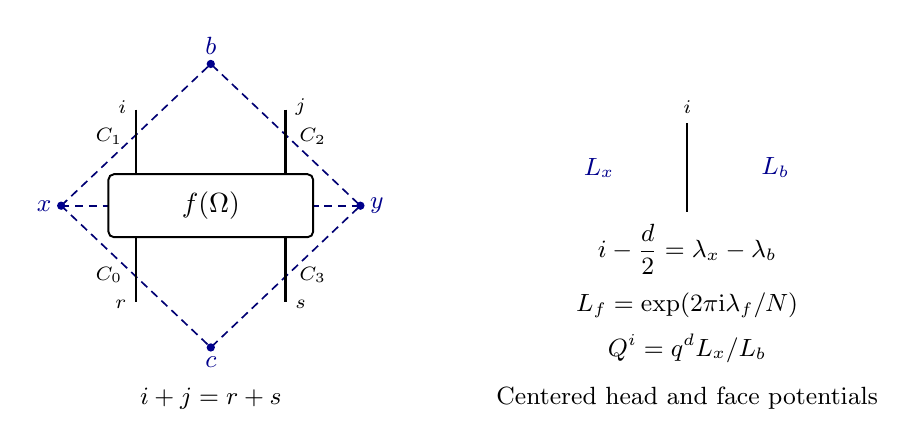
\begin{tikzpicture}[x=1cm,y=1cm,>=Latex,
  face/.style={text=blue!55!black,font=\small},
  head/.style={font=\scriptsize},
  incidence/.style={blue!45!black,densely dashed,line width=.6pt},
  strand/.style={black,line width=.8pt}]
  % White vertices record the dual faces; black curves are the two strands.
  \begin{scope}
    \coordinate (x) at (-1.9,0);
    \coordinate (b) at (0,1.8);
    \coordinate (y) at (1.9,0);
    \coordinate (c) at (0,-1.8);
    \draw[incidence] (x)--(b)--(y)--(c)--cycle;
    \draw[incidence] (x)--(y);
    \foreach \p in {x,b,y,c}{\fill[blue!55!black] (\p) circle(1.5pt);}
    \node[face,left] at (x) {$x$};
    \node[face,above] at (b) {$b$};
    \node[face,right] at (y) {$y$};
    \node[face,below] at (c) {$c$};
    \draw[strand] (-.95,1.22)--(-.95,.4);
    \draw[strand] (.95,1.22)--(.95,.4);
    \draw[strand] (-.95,-.4)--(-.95,-1.22);
    \draw[strand] (.95,-.4)--(.95,-1.22);
    \draw[fill=white,rounded corners=2pt,line width=.7pt]
       (-1.3,-.4) rectangle (1.3,.4);
    \node at (0,0) {$f(\Omega)$};
    \node[head,left] at (-.95,1.25) {$i$};
    \node[head,right] at (.95,1.25) {$j$};
    \node[head,left] at (-.95,-1.25) {$r$};
    \node[head,right] at (.95,-1.25) {$s$};
    \node[head,left] at (-1,.88) {$C_1$};
    \node[head,right] at (1,.88) {$C_2$};
    \node[head,left] at (-1,-.88) {$C_0$};
    \node[head,right] at (1,-.88) {$C_3$};
    \node[font=\small] at (0,-2.45) {$i+j=r+s$};
  \end{scope}
  \begin{scope}[shift={(6.05,0)}]
    \draw[strand] (0,1.05)--(0,-.08);
    \node[head,above] at (0,1.05) {$i$};
    \node[face] at (-1.12,.48) {$L_x$};
    \node[face] at (1.12,.48) {$L_b$};
    \node[font=\small,fill=white,inner sep=3pt] at (0,-.55)
      {$i-\dfrac d2=\lambda_x-\lambda_b$};
    \node[font=\small,align=center] at (0,-1.55)
      {$L_f=\exp(2\pi\mathrm i\lambda_f/N)$\\[5pt]
       $Q^i=q^dL_x/L_b$};
    \node[font=\small,align=center] at (0,-2.45)
      {Centered head and face potentials};
  \end{scope}
\end{tikzpicture}

 \caption{The ordered box has cyclic face order \((x,b,y,c)\) and
 polynomial \(H_f(x,b,c,y)\). Its two inputs are \(C_1,C_2\), and
 its outputs are \(C_0,C_3\). The matching diagonal \(xy\) is not a
 physical strand. On a supported state the displayed head satisfies
 \(i-d/2=\lambda_x-\lambda_b\); this fixes the sign of the face
 potential. The alternative side numbering \(0,1,2,3\) refers to
 \(C_1,C_2,C_3,C_0\).}
 \label{de:figure}
\end{figure}

A main edge means one of the edges outside the box disks. Choose one
as a marked edge and call its adjacent faces \(a,b\). They are
distinct. Indeed a connected four-valent graph has no bridge:
if removing a single edge separated a set of vertices, the sum of
their degrees would be twice the number of internal edges plus one,
contrary to its even parity. An edge incident to only one face of
a spherical graph is a bridge.

The matrices defining the turns and mark are given below. Let
\(A_{\rm raw}(f_1,\ldots,f_R)\) be their contraction, with exactly
one marked cap and with the full operators \(f_e(\Omega)\) in the
recorded boxes. Each \(f_e\) is a finite polynomial; its coefficients
may depend on \(N\) and on other parameters. In particular it may
already include a signed crossing power through
Proposition~\ref{fb:crossing-polynomial}. Set
\[
 \mathcal P(L)=\prod_{e=1}^R
 H_{f_e}(L_{x_e},L_{b_e},L_{c_e},L_{y_e}).
\]
Every local factor is homogeneous of degree \(d\), so
\(\deg\mathcal P=dR\).

\begin{theorem}[The exact marked face coefficient]
\label{de:coefficient-theorem}
For the stated ordered diagram and the full polynomial coupons,
\begin{equation}\label{de:coefficient}
 A_{\rm raw}(f_1,\ldots,f_R)
 =\left[\prod_{f\ne a,b}L_f^d\right]
       \left.\mathcal P(L)\right|_{L_a=L_b=0}.
\end{equation}
This is an identity at each level, with no omitted power of \(N\).
The reduced scalar is independent of the chosen main edge when the
cut and its duality frames are transported as below. The theorem
does not assert this independence for separate projections of a
local polynomial onto selected monomials.
\end{theorem}

We prove the theorem in several finite steps. The first concerns
the reduced cut; the remaining steps turn its state sum into the
displayed coefficient.

\subsection{Duality, turns and the unrestricted mark}

For a generic nonzero parameter \(z\) which is not a root of unity,
let \(V_L\) have basis \(v_0,\ldots,v_L\) and operators
\[
 Kv_i=z^{L-2i}v_i,\qquad
 Fv_i=v_{i+1},\qquad
 Ev_i=[i]_z[L-i+1]_zv_{i-1}.
\]
Endpoint vectors are zero. The coproducts are those used in
Section~\ref{fb:crossing}, and the antipodes are
\[
 S(E)=-EK^{-1},\qquad S(F)=-KF,\qquad S(K)=K^{-1}.
\]
The dual action is obtained by transposing these antipode matrices.
Put
\begin{equation}\label{de:J}
 J_zv_i=c_i(z)v_{L-i}^*,\qquad
 c_i(z)=(-1)^iz^{i(i-L-1)}.
\end{equation}
This is an intertwining map from \(V_L\) to its dual. For \(F\),
the required ratio is
\[
 c_{i+1}/c_i=-z^{-L+2i};
\]
the \(K\) equation reverses the weights, and the \(E\) equation then
uses the same ratio and the displayed quantum integers. These
checks also show that \(J_z\) and its inverse are regular near our
root when \(L=d\).

The integer-weight operator \(H\) satisfies \(K=z^H\). Since \(E\)
and \(F\) change weights by two, \((-1)^H\) is central and
group-like. Consequently
\[
              \widetilde g=(-1)^HK
\]
implements \(S^2\) on every tensor product and dual used here.
In the given self-dual frame it is exactly the double-dual map:
\[
 J_z^{-t}J_z=\widetilde g,\qquad
 \frac{c_i(z)}{c_{L-i}(z)}=(-1)^Lz^{L-2i}.
\]
At \(z=q\), every integral weight satisfies \(q^{-NH}=(-1)^H\).
Thus the generic pivot specializes to the physical root pivot
\begin{equation}\label{de:pivot}
                       g=K^{1-N}.
\end{equation}
This specialization uses a regular generic pivot; it does not
assert that \(K^{1-N}\) implements \(S^2\) for a generic \(z\).

Take \(L=d\) and pass to the balanced basis
\(e_i=v_i/(Q;Q)_i\) at the root. The product identity
\begin{equation}\label{de:factorial-cancellation}
 (Q;Q)_i(Q;Q)_{d-i}
       =N(-1)^iQ^{i(i+1)/2}
\end{equation}
follows from \((Q;Q)_d=N\) and
\(1-Q^{-j}=-Q^{-j}(1-Q^j)\).
Since \(c_i(q)=q^{i^2}\), the factorials in \(J_q\) therefore
cancel exactly. If the first tensor factor below is a dual factor,
denote it by a superscript \(\vee\). The four ordered turns are
\[
\begin{aligned}
 \operatorname{ev}_L(e_a^\vee\otimes e_b)
      &=N^{-1}x_0^a\,\mathbf1_{a+b=d},&
 \operatorname{coev}_L(1)
      &=\sum_a Nx_0^{-a}e_{d-a}\otimes e_a^\vee,\\
 \operatorname{ev}_R(e_b\otimes e_a^\vee)
      &=N^{-1}x_0^ag_b\,\mathbf1_{a+b=d},&
 \operatorname{coev}_R(1)
      &=\sum_a Nx_0^{-a}g_{d-a}^{-1}
                       e_a^\vee\otimes e_{d-a},
\end{aligned}
\]
where
\[
                       g_j=q^{-d^2-2j}.
\]
Contraction of a turn with the opposite turn has a single matching
index; its \(x_0\) and \(g\) factors cancel. This proves all four
snake identities. Closing an endomorphism by the corresponding
ordinary turns gives the pivotal trace \(\operatorname{Tr}(gA)\).

In literal left-to-right physical head order \((i,j)\), both cups
and both caps reduce to
\begin{equation}\label{de:root-turns}
 p_{ij}=Nq^{-d^2+di}\mathbf1_{i+j=d},
 \qquad
 \ell_{ij}=N^{-1}q^{di}\mathbf1_{i+j=d}.
\end{equation}
For example the right-cap ratio to the stated cap is
\(q^{-2Ni}=1\), and the right-cup ratio is
\(q^{2N(d-i)}=1\). These are equalities of the actual turn matrices,
not independent rescalings of the local frames.

Define the rank-one projector \(e=\psi\phi\) by
\(\psi_i=1\), \(\phi_i=1/N\), so \(e^2=e\) and
\(\operatorname{Tr}e=1\). At a right cut insert \(g^{-1}e\)
on the primal input. For every matrix \(C\),
\[
                 \operatorname{Tr}(g\,g^{-1}eC)
                           =\operatorname{Tr}(eC).
\]
At a left cut use the corresponding defect \(ge\). In physical
left-to-right order the resulting marked rows are
\begin{equation}\label{de:unrestricted-mark}
 m_R(i,j)=\frac{x_0^j}{N^2},\qquad
 m_L(i,j)=\frac{x_0^i g_{d-i}}{N^2}.
\end{equation}
For the right row, the only summand in
\(\operatorname{ev}_R(g^{-1}e\,e_i\otimes e_j^\vee)\)
has primal index \(d-j\), and its pivot times defect entry is
\(1/N\). This gives the first formula; the left formula follows
by the same single-index contraction. Neither marked row has a
support restriction.

Each complete marked cup-cap contraction is one. In a whole
closed diagram with one marked cap, conservation forces the
marked heads to satisfy \(i+j=d\): each box preserves the true
integer sum of its two indices, every cup supplies \(d\), and
every other cap consumes \(d\). On this forced support both
rows in \eqref{de:unrestricted-mark} equal
\begin{equation}\label{de:mark-on-support}
                         m_{ij}=N^{-2}q^{dj}.
\end{equation}
We shall use \eqref{de:mark-on-support} only after this global
conservation argument. Restricting the marked row in advance
would be a different tensor.

\subsection{Why the chosen reduced cut can be exposed}

We next justify moving the marked edge to an exposed top cap
while keeping every coupon disk and its ordered frame fixed.
This is the only place where a closed spherical reading of the
diagram is compared with a different planar reading.

For the generic pivot \(\widetilde g\), the two traces agree on
every intertwiner in the tensor-generated category:
\begin{equation}\label{de:spherical-traces}
 \operatorname{Tr}(\widetilde gA)
       =\operatorname{Tr}(\widetilde g^{-1}A).
\end{equation}
Here is a direct proof including multiplicity spaces. First take
real \(z>0\), \(z\ne1\). The involution
\[
                  K^*=K,\qquad E^*=KF,\qquad F^*=EK^{-1}
\]
is compatible with the stated coproducts. On \(V_L\), choose
orthogonal basis vectors with squared norms
\[
 n_0=1,\qquad
 n_i=[i]_z[L-i+1]_z\,z^{-L+2i}n_{i-1}>0.
\]
These give precisely the displayed adjoint relations. Tensor
products are unitary for the tensor-product norm; duals are
unitarized by \eqref{de:J}. An invariant subspace therefore has
an invariant orthogonal complement.

Every irreducible summand is one of the \(V_L\). Indeed choose a
highest vector \(v\) of integral weight \(L\). The identity
\[
 EF^rv=[r]_z[L-r+1]_zF^{r-1}v
\]
shows that the first zero lowering occurs at \(r=L+1\); a
negative highest weight would have no zero lowering. Bounded
weights exclude that possibility. The preceding nonzero
lowerings have distinct weights and span the irreducible
summand. An intertwiner consequently has blocks
\(I_{V_L}\otimes A_L\). On each such block both sides of
\eqref{de:spherical-traces} equal
\[
                         (-1)^L[L+1]_z\operatorname{Tr}(A_L),
\]
because the weights \(L,L-2,\ldots,-L\) are symmetric.

For a fixed diagram all matrix entries are rational in a fixed
local square root of \(z\). Polynomial coupon coefficients are
held fixed while taking this generic lift. The identity on an
interval of positive real \(z\) proves the rational identity,
and all original matrices are regular at \(q\). For the
crossing this regularity was proved in
Proposition~\ref{fb:crossing-polynomial}; its inverse is regular
as well because its root value is invertible. Thus
\eqref{de:spherical-traces} specializes to the actual diagram.
No decomposition or projection onto the generic irreducible
summands is specialized.

Choose a point in face \(a\) and move it to the point at infinity
along a path outside all coupon disks. A thin strip around that
path gives a sphere isotopy which fixes the disks pointwise.
The outside arcs may be crossed by the moving infinity, but no
crossing or ribbon twist is introduced. Ordinary portions of the
motion are tensor interchange and the four snake identities.
When infinity passes an arc, the two planar readings close the
same bent endomorphism by its two pivotal traces. Equality
\eqref{de:spherical-traces} gives the same generic closed scalar.
Face \(a\) is now exterior.

The chosen edge borders that exterior face. Push a short subarc
along a narrow strip within the face to a point above the
remaining compact drawing. Its tip is a top cap; the strip
introduces no crossing or extra component. The inside face is
still \(b\). Perturb the other arcs to make their turns Morse.

Leave the new cap open. After the actual cup identification,
the remaining diagram is an endomorphism of \(V_d\) or its dual.
Generically it is a scalar \(a(z)I\): commuting with the distinct
\(K\) weights makes it diagonal, and commuting with the nonzero
adjacent \(F\) arrows makes its diagonal constant. The scalar is
regular at \(q\), since it is an entry of a regular open network.
Closing it ordinarily gives
\[
                         (-1)^d[N]_z\,a(z).
\]
This factor is the same for every exposed cut, even on a
different component, because every component has the same
color. It is nonzero generically, so equal closed scalars have
equal regular open scalars. Specialization gives their equality
at \(q\), without division by \([N]_q=0\).
The marked closure evaluates \(\operatorname{Tr}(e\,aI)=a\).
This proves the required independence of the reduced cut.

This argument does not commute the nonintertwining defect
\(g^{-1}e\) through the boxes. It first transports the cut with
its true cups and duality, and then identifies its reduced scalar.

\subsection{The affine face lattice and the true support}

We describe the state space before evaluating the turn factors.
For a vertical head separating a left face \(f\) from a right
face \(g\), use the convention
\begin{equation}\label{de:centered-flow}
 i-\frac d2=\lambda_f-\lambda_g,\qquad
 L_f=\exp(2\pi i\lambda_f/N).
\end{equation}
At the first input of a box this reads
\(Q^i=q^dL_x/L_b=-q^{-1}L_x/L_b\), exactly the first
clock in the local Fourier proof. At the other input the ratio
is \(q^dL_b/L_y\); the two output ratios use \(c\) in place of
\(b\). Reversing an arc replaces its head \(i\) by \(d-i\),
so its centered value changes sign.

A physical state on the unmarked diagram is a choice of canonical
heads \(0,\ldots,d\). At a turn the heads sum to \(d\); at every
box the two input heads have the same integer sum as the two
output heads. Centered heads thus define an antisymmetric flow
on the edges of \(\Gamma\), with zero divergence at each vertex.
Equivalently, they give a closed cochain on the dual face graph.

For clarity, the required integral fact holds over every
abelian group. A zero-divergence flow on a connected spherical
graph is the difference of face potentials, unique after one
potential is fixed. To prove it, integrate the dual cochain from
the fixed face along dual edge paths. Two paths differ by a
closed dual walk. Splitting repeated vertices reduces that walk
to simple cycles; on the sphere each such cycle bounds a union
of dual two-cells. Its cochain sum is the sum of the divergences
at the enclosed primal vertices, hence zero. This proves
path independence. Connectedness gives uniqueness. Integration
uses only addition and subtraction, so it introduces no finite
index or determinant factor.

For odd \(N\), the centered heads are integral. Fix
\(\lambda_a=0\); their potentials are then integers. For even
\(N\), twice every centered head is odd. The corresponding
parity cochain equals one on each main edge and zero on a
matching diagonal: the boundary of each triangle has two
main edges. It is closed, and the same spherical argument over
\(\mathbb F_2\) gives unique face parities \(t_f\), with
\[
 t_a=0,\qquad t_b=1.
\]
Equivalently, the dual quadrilateral at each box has four odd
edges and opposite vertices of the same parity. The exact
potentials have the form
\begin{equation}\label{de:affine-potentials}
                  \lambda_f=p_f+\frac{t_f}{2},
                  \qquad p_f\in\mathbb Z.
\end{equation}
For odd \(N\), use \(t_f=0\) throughout. These affine lattices are
nonempty: the potential \(t_f/2\) itself gives centered flow
\((t_f-t_g)/2\), and its heads lie in the physical range.
The difference of any two lifts is an integral face potential.

Reduce the \(p_f\) modulo \(N\), with \(p_a=0\). There are exactly
\(N^{R+1}\) face-grid points
\begin{equation}\label{de:face-grid}
 L_a=1,\qquad L_f=q^{t_f}Q^{p_f}\quad(f\ne a).
\end{equation}
At every such point take the canonical head representing
\(d/2+\lambda_f-\lambda_g\) modulo \(N\). At a turn the
congruence \(i+j=d\pmod N\) forces the equality \(i+j=d\):
neither \(d-N=-1\) nor \(d+N=2N-1\) lies in \([0,2d]\).

At a box the residue total need not determine the true integer
total. This is the place where physical support is essential.
The local Fourier proposition expresses the actual residue
block as a direct sum of its true-total blocks. Hence if the
canonical input and output totals differ, the matrix entry
vanishes, and \eqref{uf:physical-local-adapter} implies
\begin{equation}\label{de:unsupported-zero}
                    H_{f_e}(L_x,L_b,L_c,L_y)=0
\end{equation}
at that grid point. The prefactor there is nonzero.

If no box violates the true total, the canonical heads form the
closed centered flow just described. Integrating it gives unique
exact potentials with \(\lambda_a=0\), and they reduce to the
given grid point. Conversely every supported canonical state
gives one grid point by this integration. Additional zeros of
a coupon merely give zero weight on both sides. We have proved
a bijection between supported states and supported grid points,
and proved that all other grid points contribute zero.

The exact potentials of a supported state, rather than arbitrary
representatives \(0,\ldots,N-1\) for the \(p_f\), are used in
intermediate half-powers. In particular at a box
\[
                 r-u=\lambda_b-\lambda_c
\]
is the canonical integer displacement, since \(b,c\) have the
same parity. Thus
\begin{equation}\label{de:coherent-adapter}
 q^{-d(r-u)}c^{-d}=(bc)^{-d/2},\qquad
 f_e(\Omega)_{r,s;u,v}
        =\frac1N\frac{H_{f_e}(x,b,c,y)}{(bc)^{d/2}}.
\end{equation}
Here each fractional power means the exponential of the exact
potential in \eqref{de:centered-flow}. At even \(N\) one has
\(q^{d(p+N)}=-q^{dp}\); the proof has not asserted otherwise.
An unsupported grid point needs no such lift, because its
product already vanishes by \eqref{de:unsupported-zero}.

\subsection{Winding, the single cut factor and coefficient extraction}

Let \(M_f\) be the number of input and output middle occurrences
of face \(f\) at the boxes. Let \(T_f\) count outside turn
occurrences positively and inside turn occurrences negatively,
temporarily treating the marked cap as ordinary.
Then
\begin{equation}\label{de:winding}
 M_f-T_f=2\quad(f\ne a),\qquad M_a-T_a=-2.
\end{equation}
Indeed traverse each face boundary with the face on its left.
Resolve repeated boundary passages by a narrow regular
neighborhood. In the recorded local box resolution each middle
passage reverses the vertical tangent and contributes \(\pi\);
the two outer passages have net turn zero. An inside cup or cap
contributes \(\pi\), and its outside passage contributes
\(-\pi\). The intervening monotone arcs have zero net contribution
after deformation to vertical tangents. This also follows by
counting signed passages through a horizontal tangent direction.
The bounded-face boundary has winding \(+1\), and the exterior
boundary winding \(-1\), proving \eqref{de:winding}. Every repeated
occurrence of a face is counted, and no restriction on the
relative heights of different boxes was used.

At a cup or cap with outside face \(o\) and inside face \(z\),
the first head satisfies
\[
 q^{di}=q^{d^2/2}(L_o/L_z)^{d/2}.
\]
Thus an ordinary cup contributes \(Nq^{-d^2/2}\) times this
face character and a cap contributes \(N^{-1}q^{d^2/2}\) times
the same character. There are equally many cups and caps, so
their constant phases and powers of \(N\) cancel before one cap
is marked. At that exposed cap, \eqref{de:mark-on-support} gives
\begin{equation}\label{de:mark-ratio}
 \frac{m_{ij}}{\ell_{ij}}
      =N^{-1}q^{d(j-i)}
      =N^{-1}(L_b/L_a)^d.
\end{equation}
Equations \eqref{de:coherent-adapter} and \eqref{de:winding}
therefore turn the whole literal marked summand into
\begin{equation}\label{de:marked-summand}
 N^{-R-1}\,
       \frac{\mathcal P(L)}{\prod_{f\ne a,b}L_f^d}.
\end{equation}
Equivalently, with \(k\) cups, \(k-1\) ordinary caps and one
marked cap, the turn count is
\(N^kN^{-(k-1)}N^{-2}=N^{-1}\); each of the \(R\) local Fourier
inversions supplies its separate \(N^{-1}\).
This is the single reduced-cut normalization.

All fractional face powers have disappeared from
\eqref{de:marked-summand}. Changing any exact potential by a
multiple of \(N\) leaves this whole expression unchanged. By
the supported-state argument it can be summed over the entire
grid \eqref{de:face-grid}, not just over a chosen lift.

It remains to calculate this normalized grid average.
A monomial of \(\mathcal P\) has nonnegative face exponents \(n_f\)
with total \(dR\). Character orthogonality on each of the
\(R+1\) independent \(N\)-point grids gives the conditions
\[
 n_b\equiv0\pmod N,\qquad n_f\equiv d\pmod N
                       \quad(f\ne a,b).
\]
There are \(R\) ordinary faces, each with exponent at least \(d\).
Their minimum already exhausts the total degree \(dR\).
Consequently the only surviving exponents are
\begin{equation}\label{de:unique-target}
             n_a=n_b=0,\qquad n_f=d\quad(f\ne a,b).
\end{equation}
At this exponent the even-coset character is exactly one.
The \(N^{R+1}\) grids cancel the denominator in
\eqref{de:marked-summand}. This proves
Theorem~\ref{de:coefficient-theorem}, with both parities and the
entire normal data of every coupon retained.

\subsection{Insertion of signed powers after the shared extraction}

The preceding theorem is an equality for full polynomial
operators. It may therefore be combined with resolvent
reproduction before any estimate is taken. Define
\begin{equation}\label{de:shared-numerator}
 S_N(\boldsymbol\sigma)=
 \left[\prod_{f\ne a,b}L_f^d\right]
 \left.
 \prod_{e=1}^R H_{V_N(\sigma_e;\Omega)}
        (L_{x_e},L_{b_e},L_{c_e},L_{y_e})
 \right|_{L_a=L_b=0}.
\end{equation}
Each spectral degree is at most \(d\). The extraction and
multiplication in \eqref{de:shared-numerator} take place in the
same face variables as in the original diagram.

\begin{corollary}[Exact filling of the marked source]
\label{de:exact-filling}
For any fixed signed integer powers \(n_1,\ldots,n_R\), the
raw marked evaluation with \(B_q^{n_e}\) in box \(e\) is
\begin{equation}\label{de:tensor-filling}
 A_{\rm raw}(\boldsymbol n)
       =\left(\bigotimes_{e=1}^R\mathcal L_N^{n_e}\right)
                                        S_N(\boldsymbol\sigma).
\end{equation}
If \(C_N\) is any other polynomial with the same separate spectral
degree bound, then
\[
 \left|A_{\rm raw}(\boldsymbol n)
       -\left(\bigotimes_e\mathcal L_N^{n_e}\right)C_N\right|
 \le\prod_e(1+|n_e|/2)\,
                   \|S_N-C_N\|_{[-2,2]^R}.
\]
The joint-grid improvement of Theorem~\ref{fb:main} applies when
its vanishing hypothesis is satisfied.
\end{corollary}

\begin{proof}
Proposition~\ref{prop:resolvent-reproduction} gives
\(\mathcal L_N^{n_e}V_N(\sigma_e;\Omega)=
\widetilde f_{n_e}(\Omega)\) in each individual box.
Proposition~\ref{fb:crossing-polynomial} identifies the latter
with \(B_q^{n_e}\). The ordered tensor contraction is multilinear
in its local matrices, so these identities may be applied
separately at every box and then
Theorem~\ref{de:coefficient-theorem} gives
\eqref{de:tensor-filling}. No commutation between boxes is used.
Subtract the two full shared polynomials before applying
Theorem~\ref{fb:main}; this proves the norm assertion.
\end{proof}

The exact coefficient identity and the last corollary contain
no asymptotic remainder hypothesis. A strict bound for the
particular polynomial \(S_N-C_N\), and any nonzero limiting
contribution assigned to \(C_N\), remain separate analytic
questions.


\section{Comparison with the reduced Kashaev invariant}
\label{de:normalization-section}

We specify the invariant convention rather than leaving a phase or
a change of basis implicit. This comparison is finite and applies
at every \(N\ge2\). The global coefficient theorem above is used
only at \(N\ge3\).

Let \(\mathsf P\) exchange tensor factors. In this section set
\(R=\mathscr R_q\) and \(B=B_q=\mathsf P R\), using the
crossing defined in Section~\ref{fb:crossing}. Set
\[
 p_j=\prod_{r=1}^j(1-Q^r),\qquad
 \bar p_j=\prod_{r=1}^j(1-Q^{-r}),\qquad p_0=\bar p_0=1.
\]
For an integer \(a\), let \([a]_N\) be its representative in
\(\{0,\ldots,d\}\). The enhanced Kashaev crossing in the
column-vector convention is
\begin{equation}\label{de:K-crossing}
 \begin{aligned}
 (B_K)_{ce,ab}&=
 \frac{NQ^{1+c-b+(a-e)(c-b)}
       \mathbf1_{u+t<N}\mathbf1_{v+h<N}}
      {p_u\bar p_vp_t\bar p_h},\\
 (u,v,t,h)&=([b-a-1]_N,[a-c]_N,[c-e]_N,[e-b]_N).
 \end{aligned}
\end{equation}
Its enhancement is
\[
 \mu_K=-qS,\qquad \alpha_K=-q,\qquad \beta_K=1,
 \qquad Sv_j=v_{[j+1]_N}.
\]
These are the enhanced crossing and normalization of
Murakami--Murakami~\cite[\S\S1,4]{MurakamiMurakami2001}, with
their quantum parameter equal to \(Q\).
A negative braid generator uses the actual inverse of
\eqref{de:K-crossing}. The reduced value is obtained by cutting
one strand, taking the \(\mu_K\)-weighted traces on the others,
and multiplying by \(\alpha_K^{-w}\), where \(w\) is the
writhe of the braid word. Its unknot value is one.
We use the standard enhanced ribbon invariant defined by these
data; the calculation below proves the normalization comparison
rather than invoking its comparison theorem.

\begin{theorem}[Exact normalization of the marked coefficient]
\label{de:invariant-normalization}
In the enhanced braid conventions just specified, a link \(L\)
with \(c\) components satisfies
\begin{equation}\label{de:enhanced-comparison}
 F_N^g(L)=(-1)^{d(c-1)}K_N(L),
 \qquad g=K^{1-N},
\end{equation}
where \(F_N^g\) is the reduced \(g\)-pivotal evaluation normalized
by its positive curl. For a knot the sign is one.

For a diagram \(D\) of a knot \(K\) in
Theorem~\ref{de:coefficient-theorem}, with its boxes filled by
the specified signed crossing powers, the zero-framed reduced
invariant is
\begin{equation}\label{de:raw-invariant}
 K_N(K)=\zeta_{N,D}A_{\rm raw}(\boldsymbol n),
              \qquad |\zeta_{N,D}|=1.
\end{equation}
The character \(\zeta_{N,D}\) consists of the recorded integer
framing corrections. For a closed braid of writhe \(w\) in the
same convention, it is \(\theta^{-w}\), where
\(\theta=q^{-d^2/2}\).
Consequently the right side of \eqref{de:tensor-filling}, with
this same character, evaluates the original invariant.
\end{theorem}

\begin{proof}
We first compare the matrices, keeping all factorial changes
of basis. Define \(R^o=(\mathsf P B_K)^{\mathsf T}\) and the
Fourier matrix \(\mathsf F_{ij}=Q^{ij}/\sqrt N\). Put
\[
 A=(\mathsf F^{-1}\otimes\mathsf F^{-1})R^o
                         (\mathsf F\otimes\mathsf F).
\]
We claim that its only nonzero entries are
\begin{equation}\label{de:triangular-Fourier}
 A_{a-k,b+k;\,a,b}
   =Q^{1+(a-k)(b+1)}
      \frac{p_a p_{b+k}}{p_{a-k}p_b p_k},
 \qquad 0\le k\le\min(a,d-b).
\end{equation}
In particular the conservation is equality of integer sums.

Here is the finite calculation. For a nonzero entry of \(R^o\)
introduce the residues
\[
 u=[j-i-1]_N,\quad v=[i-l]_N,\quad
 t=[l-k]_N,\quad h=[k-j]_N.
\]
The two indicators say \(u+t<N\) and \(v+h<N\); their total
is congruent to \(-1\) modulo \(N\), so
\(u+v+t+h=d\). Conversely this composition and one free index
\(j\) determine the original entry:
\[
 i=j-1-u,\quad k=j+h,\quad l=j+h+t\pmod N,\qquad
 (R^o)_{ij,kl}
 =\frac{NQ^{1-(t+h)(u+h)}}{p_u\bar p_vp_t\bar p_h}.
\]
Summing the free index in the Fourier transform gives the
modular conservation delta. If
\[
 S_r(X)=\sum_{j=0}^r\frac{X^j}{p_j\bar p_{r-j}},
\]
the remaining sum is
\begin{equation}\label{de:Fourier-sum}
 A_{c,e;\,a,b}
 =\mathbf1_{a+b\equiv c+e\pmod N}
 \sum_{z=0}^d Q^{1+c-z^2+z(a+b)}
             S_{d-z}(Q^{c-z})S_z(Q^{z-a}).
\end{equation}
Use
\(\bar p_r=(-1)^rQ^{-r(r+1)/2}p_r\).
Comparing coefficients in
\((1-Q^r)S_r(X)=(X-Q^r)S_{r-1}(X)\) proves
\[
                    S_r(X)=\frac{\prod_{j=1}^r(X-Q^j)}{p_r}.
\]
The two factors in \eqref{de:Fourier-sum} now force
\(c\le z\le a\). With \(k=a-c\), the surviving sum is
\[
 Q^{1+c(b+1)}\frac{p_a}{p_c}
 \sum_{j=0}^k
   \frac{(-1)^jQ^{j(j-1)/2}Q^{(b+1)j}}{p_jp_{k-j}}
 =
 Q^{1+c(b+1)}\frac{p_a}{p_c}
                    \frac{(Q^{b+1};Q)_k}{p_k}.
\]
Here \((a;Q)_k=\prod_{r=0}^{k-1}(1-aQ^r)\), with empty
product one. The last equality is the same finite product identity after
reversing its coefficients. If \(b+k\ge N\), the numerator
contains \(1-Q^N\) and is zero. Otherwise
\((Q^{b+1};Q)_k=p_{b+k}/p_b\). This proves
\eqref{de:triangular-Fourier} with its endpoint support.

Define diagonal matrices and a scalar by
\[
 G_j=\frac{p_j}{(1-Q)^j}=q^{j(j-1)/2}[j]_q!,
 \qquad D_j=(-q)^j,\qquad \gamma=Qq^{-d^2/2}.
\]
The coefficient of \(E^k\otimes F^k\) in the defining finite
\(R\) has the factorial ratio
\(([a]_q!/[a-k]_q!)^2/[k]_q!\).
Substitute \(p_j=(1-Q)^jq^{j(j-1)/2}[j]_q!\), together with its
Cartan factor. The resulting entry is exactly
\eqref{de:triangular-Fourier}, giving
\begin{equation}\label{de:factorial-similarity}
 A=\gamma(DG\otimes G)R
                 (G^{-1}\otimes G^{-1}D^{-1}).
\end{equation}
For example, at the entry in
\eqref{de:triangular-Fourier} the multiplier is
\(\gamma D_{a-k}G_{a-k}G_{b+k}/(G_aG_bD_b)\).
This fixes the positions of the factorial gauges; no estimate
on their condition numbers has been used.

The Fourier calculation involves a transposed crossing. To
compare it with the paper's \(B=\mathsf P R\), regard the
root self-duality as the antidiagonal matrix
\[
 Jv_j=c_jv_{d-j},\qquad
 c_j=(-1)^jq^{j(j-N)}.
\]
It obeys \(JKJ^{-1}=K^{-1}\) and
\begin{equation}\label{de:transpose-bridge}
 (J\otimes J)R(J^{-1}\otimes J^{-1})=R^{\mathsf T}.
\end{equation}
For an entry shifted from \((a,b)\) to \((a+k,b-k)\),
reflection leaves the factorial ratio unchanged because
\([N-j]_q=[j]_q\). Its \(J\)-ratio is
\[
 \frac{c_{d-a-k}c_{d-b+k}}{c_{d-a}c_{d-b}}
                 =q^{2k(a-b)+2k^2}.
\]
The reflected Cartan exponent is
\(H_aH_b/2+k(H_a-H_b)-2k^2\), with
\(H_a-H_b=2(b-a)\); the extra exponents cancel. This proves
\eqref{de:transpose-bridge} entry by entry, with the same
endpoint zeros.

For a braid on \(s\) strands put
\[
 U_s=(\mathsf F^{-1})^{\otimes s}
             \bigotimes_{j=1}^s(G^{-1}D^{j-1}),
 \qquad W_s=U_sJ^{\otimes s}.
\]
Transposing \eqref{de:factorial-similarity} gives the adjacent
crossing identity for \(\mathsf P R^{\mathsf T}\).
This crossing conserves the integer total, so it commutes with
\(D\otimes D\). The powers of \(D\) therefore combine into
the displayed single \(U_s\), valid at every adjacent position.
For a signed braid word \(\beta\) of writhe \(w\), one obtains
\begin{equation}\label{de:simultaneous-braid-gauge}
 \rho_K(\beta)=\gamma^w W_s\rho_B(\beta)W_s^{-1},
 \qquad
 W_sK^{\otimes s}W_s^{-1}=\mu_K^{\otimes s}.
\end{equation}
For the enhancement identity, \(G,D\) commute with \(K^{-1}\),
\(q^{-d}=-q\), and
\(\mathsf F^{-1}\operatorname{diag}(Q^j)\mathsf F=S\).
Negative generators are handled by inverting the same
adjacent-generator identity.

We give the cut-scalar argument explicitly. For an intertwiner
\(T\) of a tensor prefix with one last factor, set
\(C=\operatorname{Tr}_{\rm last}((I\otimes K)T)\).
The ordinary last trace of
\([T,E_{\rm prefix}\otimes K+I\otimes E]=0\)
gives \([C,E_{\rm prefix}]=0\). The \(K\)-weighted last trace
of the corresponding \(F\) equation gives
\([C,F_{\rm prefix}]=0\): its other two terms cancel by
cyclicity, using
\[
 T(K_{\rm prefix}^{-1}\otimes I)
 =(K_{\rm prefix}^{-1}\otimes K^{-1})T(I\otimes K).
\]
Commutation with the prefix \(K\) is immediate. The argument
can be iterated. Once only \(V_d\) remains, its distinct \(K\)
weights and nonzero adjacent \(F\) arrows force the cut
operator to be scalar.

In particular the enhanced partial traces of the crossing are
\begin{equation}\label{de:enhancement-traces}
 \operatorname{Tr}_2(B^{\pm1}(I\otimes K))
       =\alpha^{\pm1}I,\qquad
 \alpha=q^{(N^2-1)/2},\qquad \gamma\alpha=-q=\alpha_K.
\end{equation}
For the positive trace, evaluate on \(v_0\): only the input
pair \((0,0)\) contributes. For the inverse, evaluate on
\(v_d\): only \((d,d)\) contributes. Their values are
\(q^{d^2/2+d}\) and its inverse, which proves the formula.
These inverse calculations can also be read from
\[
 R^{-1}=
 \left(\sum_{k=0}^d
   \frac{(-1)^kq^{-k(k-1)/2}(q-q^{-1})^k}{[k]_q!}
                           E^k\otimes F^k\right)
                             q^{-H\otimes H/2}.
\]
The finite binomial identity makes its two polynomial factors
multiply to one below degree \(N\), and
\((E\otimes F)^N=0\).

Now take the \(K\)-weighted traces of every strand of a braid
closure except the chosen first one. Its cut operator \(C_B\)
is scalar by the preceding argument, irrespective of the number
of link components. In \eqref{de:simultaneous-braid-gauge},
all conjugations on traced factors cancel by cyclicity.
The remaining conjugation cancels because \(C_B\) is scalar.
Equation \eqref{de:enhancement-traces} cancels every writhe
factor, so
\begin{equation}\label{de:reduced-comparison}
                    \alpha_K^{-w}C_K=\alpha^{-w}C_B.
\end{equation}
Thus the comparison is exact even when a factorial gauge is
large, and it holds at even and composite levels.

Finally change from the \(K\)-pivot to the pivot of the marked
source. At completeness
\[
                   g=(-1)^dK,\qquad
 \theta=(-1)^d\alpha=q^{-d^2/2},\qquad |\theta|=1.
\]
For an \(s\)-strand closure the \(s-1\) traced factors contribute
\((-1)^{d(s-1)}\), and the curl normalization contributes
\((-1)^{-dw}\). If the closure has \(c\) components, its braid
permutation gives \(w\equiv s-c\pmod2\). Combining these signs
with \eqref{de:reduced-comparison} proves
\eqref{de:enhanced-comparison}. The turns and marked scalar
are exactly those already computed in
\eqref{de:root-turns}--\eqref{de:mark-on-support}.
For the same framed tangle, its planar ribbon reading and its
braid reading evaluate the same specified ribbon invariant.
The actual reduced cut is independent of its exposed edge by
the preceding source proof.

For a knot, correcting an integer framing multiplies the raw
scalar by the corresponding power of the unit \(\theta\);
the component sign is one. This gives
\eqref{de:raw-invariant}. For links with separately prescribed
component framings, retain those integer twist corrections
rather than replacing them by the total writhe, which also
counts crossings between different components.
\end{proof}

The full one-cut modified convention has a further, separate
normalization. If its modified dimension is defined by
\[
 d_N(\alpha)=-q^{N(1-N)/2}
 \frac{q^{\alpha+1}-q^{-\alpha-1}}
      {q^{N\alpha}-q^{-N\alpha}},
\]
then \(M=-q q^\alpha=e^u\), with the lift
\(\alpha=d+u/\log q\), gives the whole germ
\begin{equation}\label{de:modified-dimension}
 \begin{aligned}
 d_N\!\left(d+\frac{u}{\log q}\right)
   &=i^{N+3}\frac{\sinh u}{\sinh Nu},\\
 \lim_{u\to0}d_N\!\left(d+\frac{u}{\log q}\right)
   &=\frac{i^{N+3}}N.
 \end{aligned}
\end{equation}
The value at \(u=0\) is removable. It is attached once, to the
selected cut component, and not to every auxiliary circle.
This alternative convention is not used to change the
normalization in \eqref{de:raw-invariant}.


\section{Application after a shared coefficient extraction}
\label{fb:application}

Let $L_1,\ldots,L_s$ be auxiliary variables and let
$\mathcal C$ be a fixed coefficient extraction in those variables,
possibly after some have been set to zero. Suppose the local spectral
factors $P_e(L;\sigma_e)$ have degree at most $d$ in $\sigma_e$.
Then
\[
 S_N(\boldsymbol\sigma)=\mathcal C\!\left(\prod_eP_e(L;\sigma_e)\right)
\]
has the same separate degree bounds. Theorem~\ref{fb:main} applies to
this shared polynomial itself. It does not replace the extraction by
independent maxima of its local factors.

\begin{corollary}[Exact-source implication]\label{fb:source-application}
Assume a scalar contraction $Z_N(\boldsymbol n)$ has the exact identity
\begin{equation}\label{fb:source-hypothesis}
 Z_N(\boldsymbol n)
  =\left(\bigotimes_e\mathcal L_N^{n_e}\right)S_N.
\end{equation}
Let $C_N$ be any other shared polynomial with the same separate degree
bounds, and let $Z_{N,C}=(\bigotimes_e\mathcal L_N^{n_e})C_N$. Then
\[
 |Z_N-Z_{N,C}|\le
       \prod_e(1+|n_e|/2)\,\|S_N-C_N\|_{[-2,2]^r}.
\]
If $S_N-C_N$ vanishes on the product node grid, the smaller constant
in \eqref{uf:eq-4} applies.
\end{corollary}
\begin{proof}
The finite functional is linear. Subtract \eqref{fb:source-hypothesis}
and the definition of $Z_{N,C}$ before applying \eqref{uf:eq-3} with
$J=\varnothing$, or \eqref{uf:eq-4}. This preserves the full difference,
including every source sector and all shared coefficient demands.
\end{proof}

For the intended Morse-diagram application, the local factor is the
homogeneous representation of
\[
 V_N(\sigma;\Omega)
       =\frac{\chi_N(\sigma)-\chi_N(\Omega)}{\sigma-\Omega},
\]
where the fraction is polynomial division. The Fourier calculation in
Section~\ref{uf:local-fourier} proves the local adapter and the
annihilator needed by resolvent reproduction. Proposition~\ref{fb:crossing-polynomial} also identifies the defined
finite crossing, including its repeated-root derivatives.
For the matched spherical diagrams of Section~\ref{de:section},
Corollary~\ref{de:exact-filling} proves
\eqref{fb:source-hypothesis} for the original marked contraction.
Theorem~\ref{de:invariant-normalization} then gives its reduced Kashaev
normalization when the main link is a knot. The conditional formulation
of Corollary~\ref{fb:source-application} also permits its use with other
sources whose exact evaluation has been established separately.

Here is the resulting asymptotic implication, recorded to make clear
which estimate an application must supply. It is an elementary
consequence of a strict remainder gap, not an additional source theorem.

\begin{proposition}[Transfer of a strict remainder gap]\label{fb:rate-transfer}
Fix the number of variables and the integer tuple $\boldsymbol n$.
Suppose \eqref{fb:source-hypothesis} holds and, for some real $\Phi$ and
$\eta>0$,
\[
 \|S_N-C_N\|_{[-2,2]^r}
       \le \exp\bigl(N(\Phi-\eta)+o(N)\bigr).
\]
Suppose separately that
\[
 Z_{N,C}=a_Ne^{NA},\qquad a_N\ne0\text{ eventually},\qquad
 \frac1N\log|a_N|\longrightarrow0,
 \qquad \operatorname{Re}A>\Phi-\eta.
\]
Then $Z_N$ is eventually nonzero and
\[
             \frac1N\log|Z_N|\longrightarrow\operatorname{Re}A.
\]
Multiplication by a specified scalar sequence $u_N$ with $u_N\ne0$
eventually and $N^{-1}\log|u_N|\to0$ preserves the conclusion.
\end{proposition}
\begin{proof}
The filling constant in Corollary~\ref{fb:source-application} is
independent of $N$. Let $b=\Phi-\eta$ and choose $\epsilon>0$ with
$b+2\epsilon<\operatorname{Re}A$. For all sufficiently large $N$,
\[
 |Z_N-Z_{N,C}|\le e^{N(b+\epsilon)},\qquad
 |Z_{N,C}|\ge e^{N(\operatorname{Re}A-\epsilon)}.
\]
Their ratio is at most $e^{-N(\operatorname{Re}A-b-2\epsilon)}$.
In particular it is eventually below $1/2$. The triangle and reverse
triangle inequalities give
\[
 \tfrac12|Z_{N,C}|\le|Z_N|\le\tfrac32|Z_{N,C}|.
\]
Taking logarithms and dividing by $N$ proves the limit and eventual
nonvanishing. The last assertion follows by adding
$N^{-1}\log|u_N|$.
\end{proof}

A bound for the full source at the larger rate $\Phi$ would not satisfy
this proposition when $\operatorname{Re}A<\Phi$. Nor does a leading
term for $C_N$ estimate the omitted source. These two inputs have to be
proved separately for the same fixed diagram and normalization.
Identifying $2\pi\operatorname{Re}A$ with a particular hyperbolic
volume requires a further geometric argument; it is not part of the
finite functional theorem.

\begin{thebibliography}{9}
\bibitem{Hermite1878}
C. Hermite, \emph{Sur la formule d'interpolation de Lagrange
(extrait d'une lettre \`a M. Borchardt)}, Journal f\"ur die reine und
angewandte Mathematik \textbf{84} (1878), 70--79.
\href{https://doi.org/10.1515/crelle-1878-18788405}{doi:10.1515/crelle-1878-18788405}.
\bibitem{Riesz1914}
M. Riesz, \emph{Eine trigonometrische Interpolationsformel und einige
Ungleichungen f\"ur Polynome}, Jahresbericht der Deutschen
Mathematiker-Vereinigung \textbf{23} (1914), 354--368.
\href{https://gdz.sub.uni-goettingen.de/id/PPN37721857X_0023}{Digitized original volume}.
\bibitem{Kashaev1997}
R.~M. Kashaev, \emph{The hyperbolic volume of knots from the quantum
dilogarithm}, Letters in Mathematical Physics \textbf{39} (1997),
269--275. \href{https://doi.org/10.1023/A:1007364912784}{doi:10.1023/A:1007364912784}.
\bibitem{MurakamiMurakami2001}
H. Murakami and J. Murakami, \emph{The colored Jones polynomials and the
simplicial volume of a knot}, Acta Mathematica \textbf{186} (2001),
85--104. \href{https://doi.org/10.1007/BF02392716}{doi:10.1007/BF02392716}.
\end{thebibliography}
\end{document}
